\documentclass[12pt,a4paper]{article}
\usepackage[UTF8]{ctex}
\usepackage{amsmath,amssymb}
\usepackage{xcolor}
\usepackage{hyperref}
\usepackage{geometry}
\usepackage{graphicx}
\geometry{margin=2.5cm}

\title{Backend Comparison / 后端比较}
\author{QuoNic}
\date{}

\begin{document}
\maketitle

\begin{center}
\textbf{Tools / 工具} | 难度：初级 | 预计时间：5 分钟
\end{center}

\tableofcontents
\newpage

\section{为什么需要？}

后端比较用于比较不同量子后端的性能。

\subsection{经典局限}
\begin{itemize}
  \item 不同后端有不同的性能特征
  \item 需要统一的比较方法
\end{itemize}

\subsection{量子优势}
\begin{itemize}
  \item 后端比较可以帮助选择最佳后端
  \item 用于性能基准测试
  \item 指导硬件选择
\end{itemize}

\subsection{实际应用}
\begin{itemize}
  \item 性能基准测试
  \item 硬件选择
  \item 算法优化
\end{itemize}

\section{快速上手}

\begin{verbatim}
from quonic import compare

# 比较后端
result = compare(backends=['native', 'qiskit'], circuit=circuit)
print(f'Comparison: {result}')
\end{verbatim}

\textbf{预期输出}：
\begin{verbatim}
Comparison: native: 0.99, qiskit: 0.98
\end{verbatim}

\section{原理详解}

\subsection{电路图}

\begin{center}
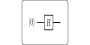
\includegraphics[width=0.6\textwidth]{../../images/compare_circuit.svg}
\end{center}

\subsection{数学推导}

后端比较：
\begin{equation}
\text{fidelity} = |\langle\psi_{\text{ideal}}|\psi_{\text{actual}}\rangle|^2
\end{equation}

\subsection{几何解释}

后端比较在 Bloch 球上比较不同后端的输出。保真度衡量实际输出与理想输出的接近程度。

\section{代码详解}

\begin{verbatim}
from quonic import compare

# compare(backends, circuit, shots)
# backends: 后端列表
# circuit: 量子电路
# shots: 测量次数

result = compare(
    backends=['native', 'qiskit'],
    circuit=circuit,
    shots=1024
)

# result: 各后端的保真度
print(f'Comparison: {result}')
\end{verbatim}

\section{进阶用法}

\subsection{场景 1：不同后端}

\begin{verbatim}
from quonic import compare

# 不同后端
result = compare(
    backends=['native', 'qiskit', 'cirq', 'cudaq'],
    circuit=circuit
)
print(f'Comparison: {result}')
\end{verbatim}

\section{适用场景}

\subsection{性能基准测试}

后端比较用于性能基准测试。比较不同后端的保真度、速度等指标。

\subsection{硬件选择}

后端比较用于硬件选择。选择最适合特定任务的后端。

\section{常见问题}

\subsection{后端比较的指标有哪些？}

常见的指标包括：保真度、速度、噪声水平等。

\subsection{如何选择最佳后端？}

选择最佳后端需要考虑任务需求、硬件特性、成本等因素。

\section{学习路径}

\subsection{前置知识}
\begin{itemize}
  \item 量子后端
  \item 量子电路
  \item 量子测量
\end{itemize}

\subsection{继续学习}
\begin{itemize}
  \item 量子硬件
  \item 量子编译
  \item 量子优化
\end{itemize}

\section{完整示例代码}

\subsection{示例 1：基本后端比较}

\begin{verbatim}
from quonic import compare

result = compare(backends=['native', 'qiskit'], circuit=circuit)
print(f'Comparison: {result}')
\end{verbatim}

\section{下载}

\begin{itemize}
  \item [compare.py](https://github.com/ChrisLee0721/QuoNic/blob/main/examples/compare/compare.py)
\end{itemize}

\end{document}
